\chapter{Introduction} \label{ch:intro}
% Word checked, no spell and gramma error. 
For any autonomous vehicle, generating an accurate and high precision model of its surrounding 
environment to indicate hazard features, and knowing its own location in the map is essential for 
the vehicle to navigate and avoid obstacle autonomously. 

In many applications, the mobile robot has a priori map. The given 
priori map may be sufficient for localization purpose, but generally do 
not have sufficent resolution or up-to-date information required for obstacle detection. Ground vehicles 
need to deal with temporary added road block and parked cars. Aerial 
vehicles may not have a high enough resolution map that indicates tall 
trees, steep hills or electrical towers. In addition, usable map does not 
always exist. Without maps and externally referenced pose information, 
the robot must produce its own map and concurrently localize itself 
within the map. This problem is referred to as the simultaneous 
localization and mapping (SLAM). 

Traditional two-dimensional SLAM algorithms are well established in the past
decade. A SLAM algorithm typically utilises measurements from several
types of sensor which can be divided into two groups, those that
provide vehicle poses and orientation measurements, such as wheel
odometer, or GPS; and those that provide landmark bearing and range
measurements, such as radar, sonar, laser range finder. In recent
years, optical sensors are actively being incorporated into SLAM
algorithm and successfully used in ground vehicle navigation. For
aerial vehicles, the experiments are mostly limited to simulation, and
results from realistic aerial video data are rare \cite{nemra_robust_2010}
\cite{jianli_unscented_2011} \cite{sunderhauf_using_2007} \cite{artieda_visual_2009}.

\section{Problem Statement}\label{section:ProblemStatement}
% Word checked.
Obstacle detection (OD) has received a lot of research interest in recent
years. Various algorithms were developed for ground, under water and
aerial vehicle using different sensors such as sonar, radar, LIDAR, and
vision. Most OD system focus on only one sensor. Yet, using multiple sensors produces a better
measurement than single sensor \cite{smith_approaches_2006}. On most unmanned aerial vehicle (UAV) platforms, many sensors are readily available ,such as accelerometers, gyroscope, GPS receiver, altimeter, etc.
Fully utilizing these sensors should improve the accuracy and robustness of an OD system, especially in harsh flying condition.

This thesis focuses on developing an obstacle detection system by
using a SLAM algorithm as a sensor fusion framework to integrate measurements from various sensors on a typical UAV navigation device. The type of application targeted by this work is medium size
UAV conducting low altitude terrain following flight in natural
environment. The obstacles are static objects on ground; moving
objects are not considered. Research presented in this thesis
contributes to the project of developing a mid-size UAV to perform
geological survey, carried out by Carleton University in collaborated
with Sander Geophysics Ltd., an Ottawa based company specialized in
high precision geophysical survey. To achieve high resolution data
acquisition, the UAV must be able to perform terrain following flight
with altitude from ground as low as 10 meters, and with ground speed ranging from 60
knots (30 m/s) to 100 knots (51.4 m/s). The specified rate of climb for the UAV
is 400ft of vertical rise per minutes (122 meters per
minutes) \cite{james_geosurv_2008}. A quick analysis on the UAV
specification and aerodynamic behavior reveals the detection requirement of the OD system. Assuming a tree height of 20
meters, which is the average height for oak or pine, to allow for
enough time to avoid obstacle, the UAV must be able to detect the
threat from a distance of at least 610 meters (Figure \ref{ob}). This
analysis indicates that the obstacle detection must be able to map
object up to a thousand meters from the UAV.

\begin{figure}[h]
\centering
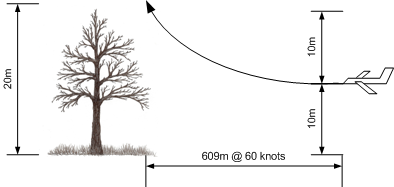
\includegraphics[width=300pt,height=160pt]{./Figures/ProblemStatement.png}
\caption {Case study for obstacle detection requirement}
\label{ob}
\end{figure}

Although digital terrain map are generally available for flight path 
planning and in flight navigation, it does not have the resolution to 
indicate all hazardous obstacle such as tall trees, steep hills, or 
man-made objects. The obstacle detection and avoidance system must 
be in place to detect discrete threat, and operate automatically with 
minimum intervene from the operator. 

\section{Contributions}\label{section:Contribution}
% word checked.
The thesis first reviewed pros and cons of various sensors, and pointed out the advantage and disadvantage of using
imaging sensor in OD application. Different types of imaging sensor
configurations and sensor calibration method was also described. Next, the
thesis reviewed the formulation and properties of a typical Extended
Kalman Filter (EKF) based SLAM algorithm, and discussed the advantage
and limitation of a typical SLAM algorithm. 

The reviews and discussions led to the development of an improved EKF SLAM
method by fusing multiple sensors with monocular camera video. 
%Using a monocular vision for mapping is a bearing only
%problem. The measurement is through projection, which loses
%information about the relative position of the feature since the range
%is unknown. Without camera motion measurements, map created by
%monocular vision can be scaled arbitrarily. 
A camera centric EKF based
SLAM algorithm (referred as CC\_EKF\_SLAM in the rest of the article)
was described in this thesis. The algorithm utilizes an extended Kalman
filter to fuse camera motion measurements from inertial and gyroscope
sensors and landmarks measurements from the video of a single wide angle
camera. Inverse parameterization was adopted to describe the landmarks
positions so that distanced landmarks can be estimated. Camera centric coordinate was used to improve the
consistency of the framework for large area mapping. The filter estimates the absolute landmarks coordinates and the position of the UAV directly. An interpolated map can be generated from the estimates to represent the surrounding environment of the UAV, and the location of the UAV within.

To test the algorithm under true flying condition, aerial flight data were collected processed by the algorithm. A simulated unmanned aerial system (SUAS) was fabricated with various sensors installed . Flight data were collected by towing the SUAS with a helicopter flying at 60 knots. The test result proved that CC\_EKF\_SLAM algorithm
is capable of mapping features over 1000 meters away. The preliminary
result of the test flight was published in \cite{zhang_obstacle_2012}.
This paper is one of the first ones in the field that successfully
applying monocular vision SLAM in large scale aerial SLAM application.
In addition, a series of simulations were done to thoroughly analyze
the behavior of the algorithm under various circumstances, including
simple forward motion, oscillatory motion for all other 5 D.O.F.,
error embedded in calibration result of the camera intrinsic
parameters, and image resolution. The results of these simulations are
valuable for the design of suitable data acquisition requirement for
obstacle detection purpose, and future improvement of the
CC\_EKF\_SLAM algorithm.

\section{Organization}\label{section:Organization}
% word checked
The thesis is organized as follows:

\begin{itemize}
  \item Chapter 2 presents an overview on sensors, and data fusion
  framework (EKF AND SLAM) related to obstacle detection and range measurement.
  \item Chapter 3 describes the detail implementation of the proposed
  CC\_EKF\_SLAM algorithm.
  \item Chapter 4 describes camera calibration procedure and result, equipments
  setup for the aerial data collection, and data preparation steps.
  \item Chapter 5 presents detail analysis on the performance of the
  algorithm. Convergence and consistency of the algorithm is
  discussed. Error analysis compared to ground truth data is presented. 
  \item Chapter 6 presents result of the simulations for understanding
  the behavior of the CC\_EKF\_SLAM algorithm under different
  conditions.  
  \item Chapter 7 gives an overall summary of the result obtained in
  this research, and a recommendation for future research items. 
\end{itemize}

%%% Local Variables:
%%% mode: latex
%%% TeX-master: "thesis.tex"
%%% End:
